\documentclass[xcolor=dvipsnames,aspectratio=169]{beamer}

% CREATED BY: Jago Cocco, Adapted by: Mattia Secchi

%\documentclass[handout,xcolor=dvipsnames,aspectratio=169]{beamer}
% Use this mode to create an handout version of the presentation to distribute to the audience:
% every "frame" will be 1 slide only, so the <onslide> commands will not influence the number of
% pages printed

%% --Packages--

\usepackage{graphicx}
%\usepackage{amsmath}
\usepackage{hyperref}
\usepackage{float}
\usepackage{geometry}
\usepackage{tikz}
\usepackage{xcolor}
%\usepackage[italian]{babel}
\usepackage{fancyhdr}

%\deftranslation[to=italian]{Example}{Esempio} %for example translation to "esempio" if needed

\mode<presentation>

%%%%%%%%%%%%%%%%%%%%%%%%%%%%%%%%%%%%%%%%%%%%%%%%%%%%%%%%%%%%%%%%%%%%%%%%%%%%%%%%%%%%%%%%%%%%%
%% Some settings...

%gets rid of bottom navigation bars and page numbers
%\setbeamertemplate{footline}{}

%gets rid of navigation symbols
\setbeamertemplate{navigation symbols}{}

%setting arev font
\usepackage{arev}

%setting geometry of blocks and shadow
\setbeamertemplate{blocks}[rounded][shadow=true]

%RGB defining color if you want manual control of color, just like RedEurac ;)
\definecolor{RedEurac}{RGB}{208,77,42} 

%general colors and scheme, fg=font color and bg=background color
%just don´t put bg={} if you don´t want a background

\setbeamercolor{structure}{fg=RedEurac,bg=White} % color of structure (itemize, enumerate...)
\setbeamercolor{section in toc}{fg=RedEurac,bg=White} % table of contents color 
\setbeamercolor{block title example}{fg=RedEurac,bg=RedEurac} %title example color
\setbeamercolor{block body example}{fg=RedEurac,bg=White} %body example color
\setbeamercolor{block title itemize}{fg=RedEurac,bg=White} %title itemize color
\setbeamercolor{block body itemize}{fg=RedEurac,bg=White} %body itemize color 
\setbeamercolor{itemize item}{fg=RedEurac,bg=white} %item colour and enumerate color
\setbeamercolor{page number in head/foot}{fg=RedEurac} %page number color
\setbeamercolor{caption name}{fg=RedEurac} %caption name color

%override color of some specific element
\setbeamercolor{frametitle}{fg=RedEurac,bg=White!20,} %frametitle color and background color
\setbeamerfont{frametitle}{series=\bfseries}
\setbeamercolor{author}{fg=RedEurac,bg={}} %author color and background color
\setbeamercolor{date}{fg=White,bg={}} %date color and background color
\setbeamercolor{title}{fg=RedEurac,bg={}} %title color and background color
\setbeamercolor{subtitle}{fg=RedEurac,bg={}} %subtitle color and background color
\setbeamercolor{footline}{fg=RedEurac,bg={}}
\setbeamerfont{footline}{series=\small}
\setbeamercolor{footnote}{fg=RedEurac}

%gets rid of the rule in the footnotes
\renewcommand*\footnoterule{}

%positions the footnote for references inside the grey box at the bottom of the page
\setbeamertemplate{footnote}{
        \hspace*{3cm}%
        \insertfootnotemark
        \parbox[b][0.5cm]{7.5cm}{
            \insertfootnotetext%
        }%
}

%\pgfpagesuselayout{4 on 1}[a4paper,border shrink=5mm,landscape]
% Activate this option if you want to insert more than one slide in each page. Landscape
% is required only for 4 and 16 slides per page

% Author info

\date{\today} %no date, just put one yourself if you want

\newcommand{\email}[1]{\href{mailto:msecchi@eurac.edu}{\emph{msecchi@eurac.edu}}}
\newcommand{\authorname}[1]{Mattia Secchi - PhD Student}
\newcommand{\institutename}[1]{Institute for Renewable Energy}
\newcommand{\affiliation}[1]{University of Trento}
\newcommand{\titledoc}[1]{100\% RES in the European grid:}
\newcommand{\subtitledoc}[1]{\emph{a new role for the consumers}}

%inserting global background, just substitute the image in the folder if you want to change it
\usebackgroundtemplate%
{%
    
\includegraphics[width=\paperwidth,height=\paperheight]{Background/middle.pdf}%
}

%inserting logo in every page after title, just substitute the images in Logo folder if you want

\addtobeamertemplate{frametitle}{}{%
\begin{tikzpicture}[remember picture,overlay]
\node[anchor=south west] at (current page.south west) {
\includegraphics[height=0.4cm]{Logo/logo.png}};
\end{tikzpicture}}

% Note: for adding a voice to summary you have to define sections with \section{•}

\begin{document}

\color{RedEurac} %setting global color of main text, you can set in here also a personalized color like RedEurac

%%%%%%%%%%%%%%%%%%%%%%%%%%%%%%%%%%%%%%%%%%%%%%%%%%%%%%%%%%%%%%%%%%%%%%%%%%%%%%%%%%%%%%%%%%%%%
%title slide

{
\usebackgroundtemplate{
\includegraphics[width=\paperwidth]{Background/front.pdf}}

\begin{frame}[noframenumbering]

\vspace{140pt}

\Large \textbf{\titledoc} \\
\normalsize \subtitledoc \\ \\
\vspace{16pt}
\authorname \\ \\
\small \affiliation

\end{frame}
}

{

\addtobeamertemplate{navigation symbols}{}{%
    \usebeamerfont{footline}%
    \usebeamercolor[fg]{footline}%
    \hspace{1em}%
    \insertframenumber/\inserttotalframenumber
    \vspace{2pt}
}

\setbeamercovered{transparent} % to have the text on the sequential slides transparent

%%%%%%%%%%%%%%%%%%%%%%%%%%%%%%%%%%%%%%%%%%%%%%%%%%%%%%%%%%%%%%%%%%%%%%%%%%%%%%%%%%%%%%%%%%%%%
% summary slide

{

\addtobeamertemplate{frametitle}{}{%
\begin{tikzpicture}[remember picture,overlay]
\node[anchor=east] at (current page.east) {
\includegraphics[height=4.5cm]{Logo/EEEIC_logo.jpg}};
\end{tikzpicture}}

\begin{frame}[t] %top for put text always in the top of the slide
\frametitle{Summary}
\vspace{-24pt}
\tableofcontents
\end{frame}

}

%inserting logos in every page after SUMMARY, just substitute the images in Logo folder if you want

\addtobeamertemplate{frametitle}{}{%
\begin{tikzpicture}[remember picture,overlay]
\node[anchor=north east] at (current page.north east) {
\includegraphics[height=2cm]{Logo/unitn.png}};
\end{tikzpicture}}

%%%%%%%%%%%%%%%%%%%%%%%%%%%%%%%%%%%%%%%%%%%%%%%%%%%%%%%%%%%%%%%%%%%%%%%%%%%%%%%%%%%%%%%%%%%%%
% Add frames here, use section to add a title in summary

\begin{section}{Nice section}
\begin{frame}[t]
\frametitle{Nice slide}
Do you want some itemize? Lets do it!
\begin{itemize}
\onslide<1->{\item Item number 1, where I want to cite something \footnote{Reference}}
%textcolor allows you to force a color in text, it is useful to set colours on itemize content
\onslide<2->{\item Item number 2}
\onslide<3->{\item Item number 3}
\end{itemize}
\end{frame}

\begin{frame}[t]
\frametitle{Nice slide with a quote}
Giving you a quote from me:
\begin{quote}
\textcolor{RedEurac}{Two things are infinite: the universe and human stupidity; and I'm not sure about the universe} %setted a personalized colour here for the quote
\end{quote} 
\end{frame}
\end{section}

\begin{section}{Another nice section!}
\begin{frame}[t]
\frametitle{Slide with an example}
\begin{example}
Hi, I am a good example, do you agree?
\end{example}
\end{frame}

\begin{frame}[t]
\frametitle{Slide with an image} 
\begin{figure}
  \centering
  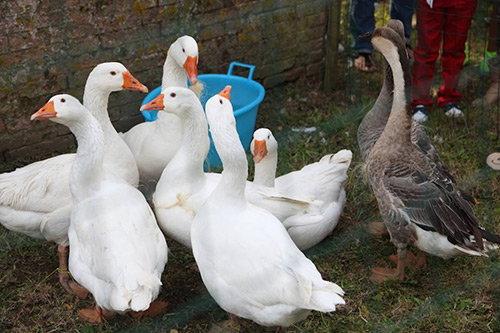
\includegraphics[scale=0.22]{Immagini/duck.jpg}
\end{figure}
\end{frame}

\begin{frame}[t]
\frametitle{Itemize with transparency}
Do you want some itemize? Lets do it!
\begin{itemize}
\onslide<1->{\item Item number 1, where I want to cite something \footnote{Reference}}
%textcolor allows you to force a color in text, it is useful to set colours on itemize content
\onslide<2->{\item Item number 2}
\onslide<3->{\item Item number 3}
\end{itemize}
\end{frame}

\end{section}

\begin{frame}[t]
\frametitle{Hyperlink slide} 
Hi, if you click \textbf{\href{https://www.google.com}{HERE}} you go on Google page 
\end{frame}

\begin{frame}
\frametitle{Slide with 2 columns, one with a picture}

\begin{columns}

\begin{column}{0.4\textwidth}
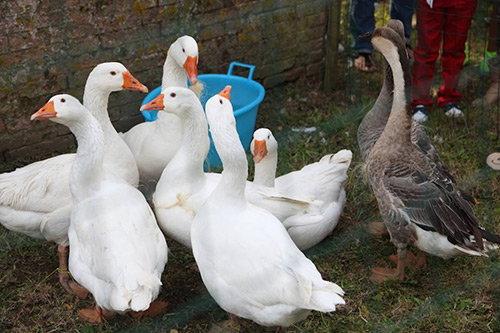
\includegraphics[width=\columnwidth]{Immagini/duck.jpg}
\end{column}

\begin{column}{0.4\textwidth}
\begin{itemize}
\item Mane
\item Tekel
\item Fares
\end{itemize}
\end{column}

\end{columns}
\end{frame}

%%%%%%%%%%%%%%%%%%%%%%%%%%%%%%%%%%%%%%%%%%%%%%%%%%%%%%%%%%%%%%%%%%%%%%%%%%%%%%%%%%%%%%%%%%%%%
% slide with some code

\begin{frame}[fragile]
\frametitle{Un algoritmo per trovare numeri primi}
\begin{verbatim}
int main (void)
{
std::vector<bool> is_prime (100, true);
for (int i = 2; i < 100; i++)
if (is_prime[i])
{
std::cout << i << " ";
for (int j = i; j < 100; is_prime [j] = false, j+=i);
}
return 0;
}
\end{verbatim}
\end{frame}

%%%%%%%%%%%%%%%%%%%%%%%%%%%%%%%%%%%%%%%%%%%%%%%%%%%%%%%%%%%%%%%%%%%%%%%%%%%%%%%%%%%%%%%%%%%%%
% bibliography (if needed)

\begin{frame}
\frametitle{\refname}
\begin{thebibliography}{9}
\bibitem{goldbach:congettura} Christian Goldbach
\newblock Un problema aperto
\newblock \emph{Lettera a Leonhard Euler}, 1742
\end{thebibliography}
\end{frame}

} % this ends the numeration

%%%%%%%%%%%%%%%%%%%%%%%%%%%%%%%%%%%%%%%%%%%%%%%%%%%%%%%%%%%%%%%%%%%%%%%%%%%%%%%%%%%%%%%%%%%%%
% Closure slide

{
\usebackgroundtemplate{
\includegraphics[width=\paperwidth]{Background/end.pdf}}

\begin{frame}[noframenumbering]

\vspace{72pt}
\huge
\textbf{Thank you \\
for your attention!} \\
\vspace{24pt}
\Large \textbf{\authorname} \\
\institutename \\ \\
\vspace{12pt}
\normalsize \email

\end{frame}
}

\end{document}